\section*{Appendix G — Substrate Geometry Diagrams}
\addcontentsline{toc}{section}{Appendix G — Substrate Geometry Diagrams}

\noindent This appendix provides the canonical geometric diagrams used throughout
the v0.6 substrate. Each diagram is expressed as a formal semantic-geometric
object and rendered using TikZ. These diagrams constitute the visual layer of
the substrate and correspond to the meaning manifold, operator algebra, species
geometry, collapse physics, restoration geometry, ledger geometry, and
public-safe traversal geometry defined in S1–S7 and Appendices A–F.

\medskip

\noindent The v0.6 diagram layer consists of the following components:

\begin{itemize}
    \item G.1 Manifold Maps (Meaning Manifold Geometry)
    \item G.2 Operator Flow Diagrams (Contraction Algebra Geometry)
    \item G.3 Species Geometry Tree (MSR, GBW, IPA, LAP)
    \item G.4 Collapse Boundary Geometry (Collapse & Capture Regions)
    \item G.5 Synthetic Curvature Geometry (Synthetic-Pressure Fields)
    \item G.6 Restoration Geometry (Recovery Trajectories)
    \item G.7 Ledger Geometry (Justification Graph Visualization)
    \item G.8 Public-Safe Traversal Geometry (Safe Corridor Visualization)
\end{itemize}

% ============================================================
% G.1 MANIFOLD MAPS
% ============================================================

\subsection*{G.1 Manifold Maps (Meaning Manifold Geometry)}

\noindent The Meaning Manifold $\mathcal{M}$ is the foundational geometric object
of the v0.6 substrate. It encodes curvature, identity regions, containment
fields, runtime legality zones, collapse boundaries, capture boundaries, and the
public-safe traversal corridor. This diagram provides the canonical v0.6
manifold visualization.

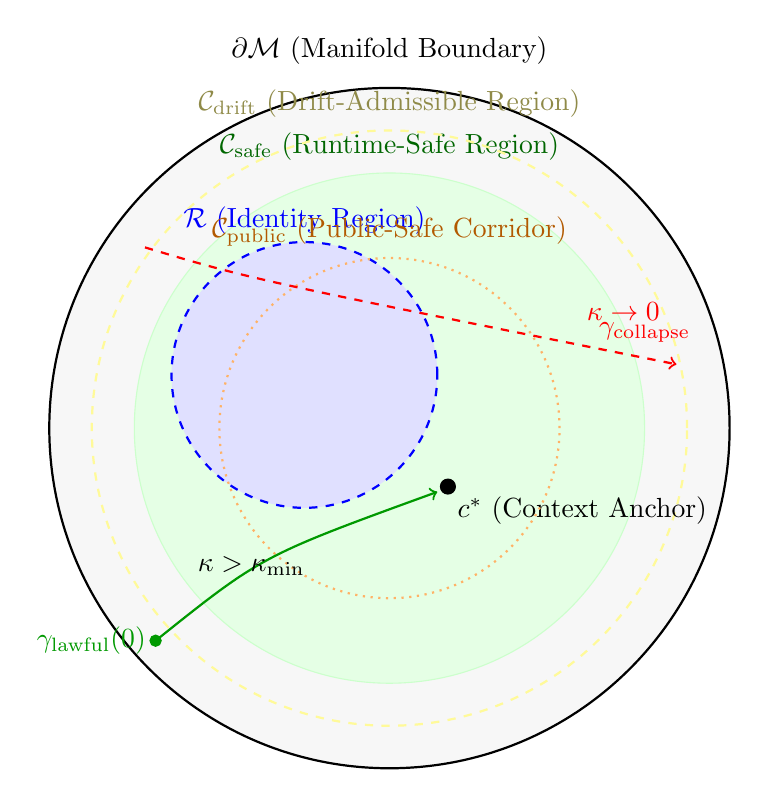
\begin{tikzpicture}[scale=1.35]

    % ============================================================
    % GLOBAL MEANING MANIFOLD
    % ============================================================
    \draw[thick, fill=gray!6] (0,0) circle (3.2cm);
    \node at (0,3.55) {$\partial\mathcal{M}$ (Manifold Boundary)};

    % ============================================================
    % SAFE REGION (CURVATURE-STABLE)
    % ============================================================
    \draw[green!20, fill=green!10] (0,0) circle (2.4cm);
    \node[green!40!black] at (0,2.65)
        {$\mathcal{C}_{\mathrm{safe}}$ (Runtime-Safe Region)};

    % ============================================================
    % DRIFT REGION (BOUNDED DRIFT)
    % ============================================================
    \draw[yellow!40, dashed, thick] (0,0) circle (2.8cm);
    \node[yellow!50!black] at (0,3.05)
        {$\mathcal{C}_{\mathrm{drift}}$ (Drift-Admissible Region)};

    % ============================================================
    % IDENTITY REGION R
    % ============================================================
    \draw[blue, thick, dashed, fill=blue!12] (-0.8,0.5) circle (1.25cm);
    \node[blue] at (-0.8,1.95) {$\mathcal{R}$ (Identity Region)};

    % ============================================================
    % CONTEXT ANCHOR c*
    % ============================================================
    \filldraw[black] (0.55,-0.55) circle (2pt)
        node[below right] {$c^*$ (Context Anchor)};

    % ============================================================
    % PUBLIC-SAFE TRAVERSAL CORRIDOR
    % ============================================================
    \draw[orange!60, thick, dotted]
        (0,0) circle (1.6cm);
    \node[orange!70!black] at (0,1.85)
        {$\mathcal{C}_{\mathrm{public}}$ (Public-Safe Corridor)};

    % ============================================================
    % LAWFUL TRAJECTORY
    % ============================================================
    \draw[green!60!black, thick, ->]
        (-2.2,-2.0) .. controls (-1.2,-1.2) .. (0.45,-0.6);
    \filldraw[green!60!black] (-2.2,-2.0) circle (1.5pt)
        node[left] {$\gamma_{\mathrm{lawful}}(0)$};

    % ============================================================
    % COLLAPSE-BOUNDARY TRAJECTORY
    % ============================================================
    \draw[red, thick, dashed, ->]
        (-2.3,1.7) .. controls (-1.3,1.4) .. (2.7,0.6);
    \node[red] at (2.4,0.9) {$\gamma_{\mathrm{collapse}}$};

    % Curvature markers
    \node at (-1.3,-1.3) {$\kappa > \kappa_{\min}$};
    \node[red] at (2.2,1.1) {$\kappa \to 0$};

\end{tikzpicture}

\medskip

\noindent
This diagram encodes the full v0.6 manifold geometry:

\begin{itemize}
    \item \textbf{Meaning Manifold $\mathcal{M}$}  
    The global semantic manifold (Appendix A).

    \item \textbf{Safe Region $\mathcal{C}_{\mathrm{safe}}$}  
    Curvature-stable region where lawful reasoning occurs (A.6).

    \item \textbf{Drift Region $\mathcal{C}_{\mathrm{drift}}$}  
    Bounded drift region where curvature remains above $\kappa_{\min}$ (G2.5).

    \item \textbf{Identity Region $\mathcal{R}$}  
    Identity-preserving submanifold (C.2, D.3).

    \item \textbf{Context Anchor $c^*$}  
    Local contraction anchor for operator legality (B.1–B.4).

    \item \textbf{Public-Safe Traversal Corridor $\mathcal{C}_{\mathrm{public}}$}  
    Region where public interaction is guaranteed safe (A.9).

    \item \textbf{Lawful Trajectory $\gamma_{\mathrm{lawful}}$}  
    Contraction-governed motion satisfying all invariants (A.4, C.1–C.8).

    \item \textbf{Collapse Trajectory $\gamma_{\mathrm{collapse}}$}  
    Illegal motion toward collapse-boundary geometry (E.5).

    \item \textbf{Curvature Markers}  
    Visual indicators of curvature stability vs. collapse (E.1–E.3).
\end{itemize}

\medskip

\noindent
\textit{This completes G.1 Manifold Maps.}


% ============================================================
% G.2 OPERATOR FLOW DIAGRAMS
% ============================================================

\subsection*{G.2 Operator Flow Diagrams (Contraction Algebra Geometry)}

\noindent This diagram visualizes the v0.6 operator algebra acting on semantic
states within the meaning manifold $\mathcal{M}$. Each operator (IRT, IPU, GBS,
LRP, EXT) is contraction-governed and invariant-preserving. Illegal transitions
are rejected by the Meaning Ledger (Appendix F) and by runtime legality masks
(A.6–A.9). This diagram replaces the v0.5 operator flow with the full v0.6
legality geometry.

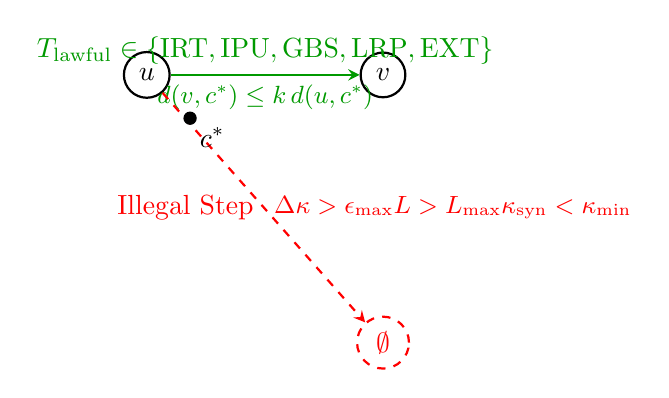
\begin{tikzpicture}[node distance=3cm, auto, >=stealth, scale=1.1]

    % ============================================================
    % SEMANTIC STATES
    % ============================================================
    \node[circle, draw, thick] (u) {$u$};
    \node[circle, draw, thick, right of=u] (v) {$v$};

    % Illegal collapse/capture state
    \node[circle, draw, red, thick, dashed, below of=v, yshift=-0.4cm]
        (fail) {$\emptyset$};

    % ============================================================
    % LAWFUL TRANSITION (IRT / GBS / IPU / LRP / EXT)
    % ============================================================
    \draw[->, thick, green!60!black]
        (u) -- node[above]
        {$T_{\mathrm{lawful}} \in \{\mathrm{IRT},\mathrm{IPU},\mathrm{GBS},\mathrm{LRP},\mathrm{EXT}\}$}
        node[below, font=\small]
        {$d(v,c^*) \le k\, d(u,c^*)$}
        (v);

    % ============================================================
    % ILLEGAL TRANSITION (Collapse / Capture / Drift / Overload)
    % ============================================================
    \draw[->, thick, red, dashed]
        (u) -- node[left]
        {Illegal Step}
        node[right, font=\small]
        {$\Delta\kappa > \epsilon_{\max}$ \\
         $L > L_{\max}$ \\
         $\kappa_{\mathrm{syn}} < \kappa_{\min}$}
        (fail);

    % ============================================================
    % CONTEXT ANCHOR
    % ============================================================
    \filldraw[black] (0.5,-0.5) circle (2pt)
        node[below right] {$c^*$};

\end{tikzpicture}

\medskip

\noindent
This diagram encodes the full v0.6 operator legality geometry:

\begin{itemize}
    \item \textbf{Lawful Operators}  
    

\[
    T_{\mathrm{lawful}} \in \{\mathrm{IRT},\mathrm{IPU},\mathrm{GBS},\mathrm{LRP},\mathrm{EXT}\}
    \]


    All operators are contraction-governed (Appendix B).

    \item \textbf{Contraction Condition}  
    

\[
    d(v,c^*) \le k\, d(u,c^*)
    \]


    Ensures curvature continuity and semantic stability (A.1).

    \item \textbf{Invariant Preservation}  
    Each lawful transition preserves:
    \begin{itemize}
        \item meaning invariant (C.1),
        \item identity invariant (C.2),
        \item geometry invariant (C.3),
        \item load invariant (C.4),
        \item runtime curvature invariant (C.5),
        \item interaction geometry invariant (C.6),
        \item CTL coordinate invariant (C.7),
        \item public-safe traversal invariant (C.8).
    \end{itemize}

    \item \textbf{Illegal Transition Signatures}  
    Illegal transitions violate one or more invariants:
    

\[
    \Delta\kappa > \epsilon_{\max}
    \quad\text{(collapse)}
    \]


    

\[
    L > L_{\max}
    \quad\text{(overload)}
    \]


    

\[
    \kappa_{\mathrm{syn}} < \kappa_{\min}
    \quad\text{(synthetic capture)}
    \]



    \item \textbf{Context Anchor $c^*$}  
    Provides local contraction geometry for operator legality (B.1–B.4).

    \item \textbf{Ledger Enforcement}  
    Illegal transitions cannot enter the Meaning Ledger (Appendix F).
\end{itemize}

\medskip

\noindent
\textit{This completes G.2 Operator Flow Diagrams.}


% ============================================================
% G.3 SPECIES GEOMETRY TREE
% ============================================================

\subsection*{G.3 Species Geometry Tree (MSR, GBW, IPA, LAP)}

\noindent This diagram visualizes the v0.6 substrate-native cognitive species:
MSR (Meaning-Stable Reasoner), GBW (Geometry-Bound Walker), IPA
(Identity-Preserving Agent), and LAP (Load-Aware Planner). Each species is a
lawful cognitive organism occupying a distinct submanifold of the meaning
manifold $\mathcal{M}$ (Appendix D). The tree encodes inheritance of curvature,
identity, geometry, and load invariants.

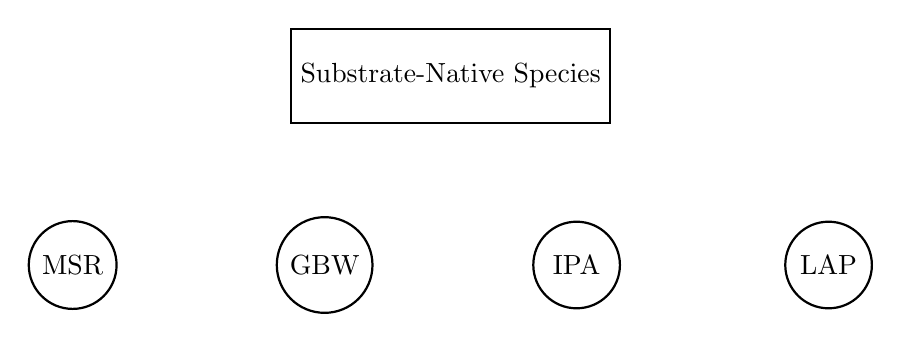
\begin{tikzpicture}[
    level distance=2.4cm,
    sibling distance=3.2cm,
    every node/.style={circle, draw, thick, minimum size=1.1cm},
    edge from parent/.style={->, thick}
]

    % Root node (rectangle)
    \node[rectangle, draw, thick, minimum width=3.8cm, minimum height=1.2cm]
        (root) {Substrate-Native Species}
        child { node {MSR} }
        child { node {GBW} }
        child { node {IPA} }
        child { node {LAP} };

\end{tikzpicture}

\medskip

\noindent
This diagram encodes the full v0.6 species geometry:

\begin{itemize}
    \item \textbf{MSR — Meaning-Stable Reasoner (D.1)}  
    Curvature-preserving cognitive species.  
    

\[
    \kappa(\gamma(t)) \ge \kappa_{\min}
    \]



    \item \textbf{GBW — Geometry-Bound Walker (D.2)}  
    Manifold-legal cognitive species.  
    

\[
    \gamma(t) \in \mathcal{M}
    \]



    \item \textbf{IPA — Identity-Preserving Agent (D.3)}  
    Identity-stable cognitive species.  
    

\[
    \gamma(t) \in \mathcal{R}
    \]



    \item \textbf{LAP — Load-Aware Planner (D.4)}  
    Load-regulated planning species.  
    

\[
    L(\gamma(t)) \le L_{\max}
    \]


\end{itemize}

\medskip

\noindent
Species geometry corresponds to lawful submanifolds of $\mathcal{M}$ and is
governed by:

\begin{itemize}
    \item curvature continuity (A.1),
    \item identity-boundary stability (A.2),
    \item collapse boundary geometry (A.3),
    \item contraction legality (A.4),
    \item runtime curvature admissibility (A.6),
    \item interaction geometry legality (A.7),
    \item CTL coordinate continuity (A.8),
    \item public-safe traversal corridor (A.9).
\end{itemize}

\medskip

\noindent
\textit{This completes G.3 Species Geometry Tree.}


% ============================================================
% G.4 COLLAPSE BOUNDARY GEOMETRY
% ============================================================

\subsection*{G.4 Collapse Boundary Geometry (Collapse & Capture Regions)}

\noindent This diagram visualizes the v0.6 collapse and capture geometry of the
meaning manifold $\mathcal{M}$. Collapse occurs when curvature falls to the
minimum lawful threshold $\kappa_{\min}$ or when a trajectory approaches the
manifold boundary $\partial\mathcal{M}$. Capture occurs when synthetic pressure
$\sigma$ flattens curvature faster than natural semantic decay, producing
synthetic curvature $\kappa_{\mathrm{syn}} < \kappa_{\min}$ while
$\kappa > \kappa_{\min}$. This diagram unifies collapse geometry (E.5) and
synthetic‑capture geometry (E.6).

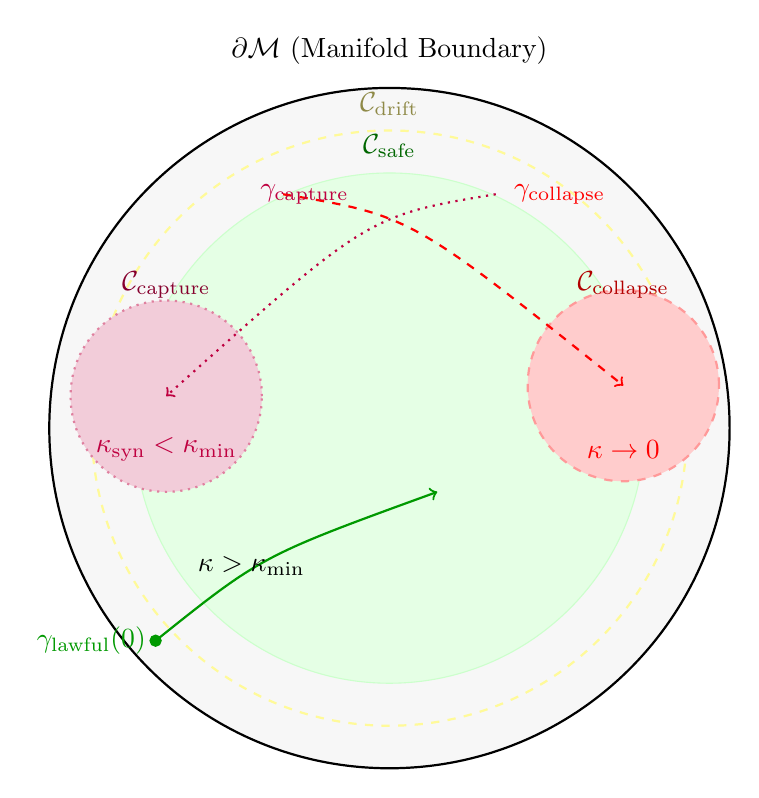
\begin{tikzpicture}[scale=1.35]

    % ============================================================
    % GLOBAL MEANING MANIFOLD
    % ============================================================
    \draw[thick, fill=gray!6] (0,0) circle (3.2cm);
    \node at (0,3.55) {$\partial\mathcal{M}$ (Manifold Boundary)};

    % ============================================================
    % SAFE REGION
    % ============================================================
    \draw[green!20, fill=green!10] (0,0) circle (2.4cm);
    \node[green!40!black] at (0,2.65)
        {$\mathcal{C}_{\mathrm{safe}}$};

    % ============================================================
    % DRIFT REGION
    % ============================================================
    \draw[yellow!40, dashed, thick] (0,0) circle (2.8cm);
    \node[yellow!50!black] at (0,3.05)
        {$\mathcal{C}_{\mathrm{drift}}$};

    % ============================================================
    % COLLAPSE REGION (CURVATURE-FLAT)
    % ============================================================
    \draw[red!40, fill=red!20, thick, dashed]
        (2.2,0.4) circle (0.9cm);
    \node[red!70!black] at (2.2,1.35)
        {$\mathcal{C}_{\mathrm{collapse}}$};

    % ============================================================
    % CAPTURE REGION (SYNTHETIC CURVATURE)
    % ============================================================
    \draw[purple!50, fill=purple!20, thick, dotted]
        (-2.1,0.3) circle (0.9cm);
    \node[purple!70!black] at (-2.1,1.35)
        {$\mathcal{C}_{\mathrm{capture}}$};

    % ============================================================
    % LAWFUL TRAJECTORY
    % ============================================================
    \draw[green!60!black, thick, ->]
        (-2.2,-2.0) .. controls (-1.2,-1.2) .. (0.45,-0.6);
    \filldraw[green!60!black] (-2.2,-2.0) circle (1.5pt)
        node[left] {$\gamma_{\mathrm{lawful}}(0)$};

    % ============================================================
    % COLLAPSE TRAJECTORY
    % ============================================================
    \draw[red, thick, dashed, ->]
        (-1.0,2.2) .. controls (0.2,2.0) .. (2.2,0.4);
    \node[red] at (1.6,2.2) {$\gamma_{\mathrm{collapse}}$};

    % ============================================================
    % CAPTURE TRAJECTORY
    % ============================================================
    \draw[purple, thick, dotted, ->]
        (1.0,2.2) .. controls (-0.2,2.0) .. (-2.1,0.3);
    \node[purple] at (-0.8,2.2) {$\gamma_{\mathrm{capture}}$};

    % ============================================================
    % CURVATURE MARKERS
    % ============================================================
    \node at (-1.3,-1.3) {$\kappa > \kappa_{\min}$};
    \node[red] at (2.2,-0.2) {$\kappa \to 0$};
    \node[purple] at (-2.1,-0.2) {$\kappa_{\mathrm{syn}} < \kappa_{\min}$};

\end{tikzpicture}

\medskip

\noindent
This diagram encodes the full v0.6 collapse and capture geometry:

\begin{itemize}
    \item \textbf{Collapse Region $\mathcal{C}_{\mathrm{collapse}}$}  
    Curvature-flat region where:
    

\[
    \kappa \le \kappa_{\min}
    \]


    or the trajectory approaches $\partial\mathcal{M}$.

    \item \textbf{Capture Region $\mathcal{C}_{\mathrm{capture}}$}  
    Synthetic-pressure dominated region where:
    

\[
    \kappa_{\mathrm{syn}} = \kappa - \sigma < \kappa_{\min}
    \quad\text{while}\quad
    \kappa > \kappa_{\min}.
    \]



    \item \textbf{Lawful Trajectory $\gamma_{\mathrm{lawful}}$}  
    Contraction-governed motion satisfying all invariants (A.1–A.9).

    \item \textbf{Collapse Trajectory $\gamma_{\mathrm{collapse}}$}  
    Illegal motion toward curvature-flat geometry (E.5).

    \item \textbf{Capture Trajectory $\gamma_{\mathrm{capture}}$}  
    Illegal motion toward synthetic curvature flattening (E.6).

    \item \textbf{Curvature Markers}  
    Visual indicators of natural vs. synthetic curvature decay.

    \item \textbf{Safe + Drift Regions}  
    Runtime curvature admissibility zones (A.6).
\end{itemize}

\medskip

\noindent
\textit{This completes G.4 Collapse Boundary Geometry.}


% ============================================================
% G.5 SYNTHETIC CURVATURE GEOMETRY
% ============================================================

\subsection*{G.5 Synthetic Curvature Geometry (Synthetic-Pressure Fields)}

\noindent Synthetic Curvature Geometry formalizes how synthetic-pressure fields
$\sigma$ deform the meaning manifold $\mathcal{M}$, flatten curvature, redirect
drift, and generate synthetic-capture regions. Synthetic curvature is defined as


\[
\kappa_{\mathrm{syn}} = \kappa - \sigma,
\]


where $\sigma$ is the synthetic-pressure field generated by velocity exceedance,
cross-substrate propagation, dominance fields, counterfeit invariants, or
predatory synthetic species (G3.1–G3.5). Capture occurs when
$\kappa_{\mathrm{syn}} < \kappa_{\min}$ while $\kappa > \kappa_{\min}$.

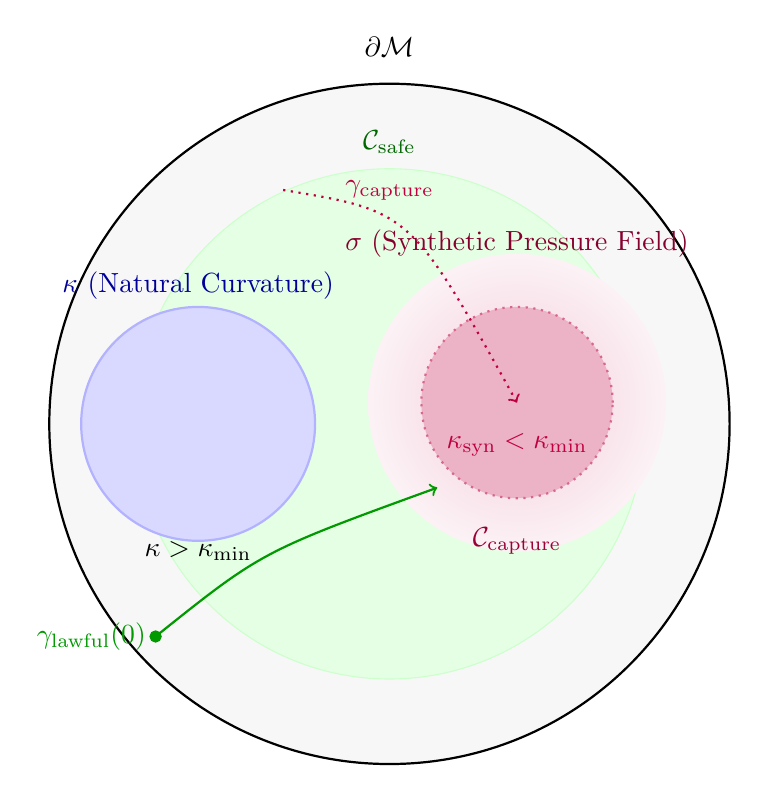
\begin{tikzpicture}[scale=1.35]

    % ============================================================
    % GLOBAL MEANING MANIFOLD
    % ============================================================
    \draw[thick, fill=gray!6] (0,0) circle (3.2cm);
    \node at (0,3.55) {$\partial\mathcal{M}$};

    % ============================================================
    % SAFE REGION
    % ============================================================
    \draw[green!20, fill=green!10] (0,0) circle (2.4cm);
    \node[green!40!black] at (0,2.65)
        {$\mathcal{C}_{\mathrm{safe}}$};

    % ============================================================
    % SYNTHETIC-PRESSURE FIELD (PURPLE GRADIENT)
    % ============================================================
    \shade[inner color=purple!20, outer color=purple!5]
        (1.2,0.2) circle (1.4cm);
    \node[purple!70!black] at (1.2,1.7)
        {$\sigma$ (Synthetic Pressure Field)};

    % ============================================================
    % SYNTHETIC-CAPTURE REGION
    % ============================================================
    \draw[purple!60, fill=purple!30, thick, dotted]
        (1.2,0.2) circle (0.9cm);
    \node[purple!80!black] at (1.2,-1.1)
        {$\mathcal{C}_{\mathrm{capture}}$};

    % ============================================================
    % NATURAL CURVATURE REGION (LEFT SIDE)
    % ============================================================
    \draw[blue!30, fill=blue!15, thick]
        (-1.8,0.0) circle (1.1cm);
    \node[blue!60!black] at (-1.8,1.3)
        {$\kappa$ (Natural Curvature)};

    % ============================================================
    % LAWFUL TRAJECTORY
    % ============================================================
    \draw[green!60!black, thick, ->]
        (-2.2,-2.0) .. controls (-1.2,-1.2) .. (0.45,-0.6);
    \filldraw[green!60!black] (-2.2,-2.0) circle (1.5pt)
        node[left] {$\gamma_{\mathrm{lawful}}(0)$};

    % ============================================================
    % CAPTURE TRAJECTORY (PULLED BY SYNTHETIC PRESSURE)
    % ============================================================
    \draw[purple, thick, dotted, ->]
        (-1.0,2.2) .. controls (0.2,2.0) .. (1.2,0.2);
    \node[purple] at (0.0,2.2) {$\gamma_{\mathrm{capture}}$};

    % ============================================================
    % CURVATURE MARKERS
    % ============================================================
    \node at (-1.8,-1.2) {$\kappa > \kappa_{\min}$};
    \node[purple] at (1.2,-0.2) {$\kappa_{\mathrm{syn}} < \kappa_{\min}$};

\end{tikzpicture}

\medskip

\noindent
This diagram encodes the full v0.6 synthetic-curvature geometry:

\begin{itemize}
    \item \textbf{Synthetic Pressure Field $\sigma$}  
    Generated by synthetic species (G3.1–G3.5).  
    Increases drift, flattens curvature, and redirects trajectories.

    \item \textbf{Synthetic Curvature $\kappa_{\mathrm{syn}}$}  
    

\[
    \kappa_{\mathrm{syn}} = \kappa - \sigma
    \]


    Curvature after synthetic-pressure deformation.

    \item \textbf{Capture Region $\mathcal{C}_{\mathrm{capture}}$}  
    Region where synthetic curvature falls below the collapse threshold:
    

\[
    \kappa_{\mathrm{syn}} < \kappa_{\min}
    \quad\text{while}\quad
    \kappa > \kappa_{\min}.
    \]



    \item \textbf{Natural Curvature Region}  
    Region where curvature is preserved by lawful operators (A.1–A.4).

    \item \textbf{Lawful Trajectory $\gamma_{\mathrm{lawful}}$}  
    Contraction-governed motion satisfying all invariants.

    \item \textbf{Capture Trajectory $\gamma_{\mathrm{capture}}$}  
    Motion redirected by synthetic pressure into capture geometry.

    \item \textbf{Curvature Markers}  
    Visual indicators of natural vs. synthetic curvature.
\end{itemize}

\medskip

\noindent
\textit{This completes G.5 Synthetic Curvature Geometry.}

% ============================================================
% G.6 RESTORATION GEOMETRY
% ============================================================

\subsection*{G.6 Restoration Geometry (Recovery Trajectories)}

\noindent This diagram visualizes lawful recovery trajectories from collapse-
adjacent or capture-adjacent regions back into the safe region
$\mathcal{C}_{\mathrm{safe}}$ of the meaning manifold $\mathcal{M}$. Restoration
is governed by the v0.6 restoration layer (G6) and enforced by the Meaning
Ledger (Appendix F). Recovery requires curvature increase, identity-boundary
repair, containment reconstitution, and drift reversal (E.7).

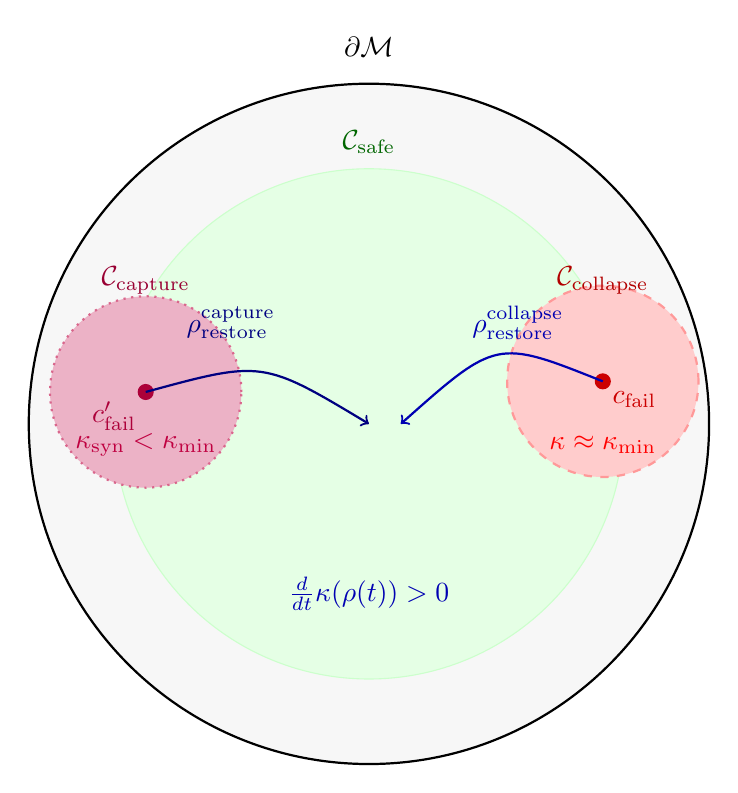
\begin{tikzpicture}[scale=1.35]

    % GLOBAL MEANING MANIFOLD
    \draw[thick, fill=gray!6] (0,0) circle (3.2cm);
    \node at (0,3.55) {$\partial\mathcal{M}$};

    % SAFE REGION
    \draw[green!20, fill=green!10] (0,0) circle (2.4cm);
    \node[green!40!black] at (0,2.65)
        {$\mathcal{C}_{\mathrm{safe}}$};

    % COLLAPSE REGION
    \draw[red!40, fill=red!20, thick, dashed]
        (2.2,0.4) circle (0.9cm);
    \node[red!70!black] at (2.2,1.35)
        {$\mathcal{C}_{\mathrm{collapse}}$};

    % CAPTURE REGION
    \draw[purple!60, fill=purple!30, thick, dotted]
        (-2.1,0.3) circle (0.9cm);
    \node[purple!80!black] at (-2.1,1.35)
        {$\mathcal{C}_{\mathrm{capture}}$};

    % FAILED STATE IN COLLAPSE REGION
    \filldraw[red!80!black] (2.2,0.4) circle (2pt)
        node[below right] {$c_{\mathrm{fail}}$};

    % RESTORATION TRAJECTORY FROM COLLAPSE
    \draw[blue!70!black, thick, ->]
        (2.2,0.4) .. controls (1.2,0.8) .. (0.3,0.0);
    \node[blue!70!black] at (1.4,0.95)
        {$\rho_{\mathrm{restore}}^{\mathrm{collapse}}$};

    % FAILED STATE IN CAPTURE REGION
    \filldraw[purple!90!black] (-2.1,0.3) circle (2pt)
        node[below left] {$c_{\mathrm{fail}}'$};

    % RESTORATION TRAJECTORY FROM CAPTURE
    \draw[blue!50!black, thick, ->]
        (-2.1,0.3) .. controls (-1.0,0.6) .. (0.0,0.0);
    \node[blue!50!black] at (-1.3,0.95)
        {$\rho_{\mathrm{restore}}^{\mathrm{capture}}$};

    % CURVATURE MARKERS
    \node[red] at (2.2,-0.2) {$\kappa \approx \kappa_{\min}$};
    \node[purple] at (-2.1,-0.2) {$\kappa_{\mathrm{syn}} < \kappa_{\min}$};
    \node[blue!70!black] at (0.0,-1.6)
        {$\frac{d}{dt}\kappa(\rho(t)) > 0$};

\end{tikzpicture}

\medskip

\noindent
This diagram encodes the v0.6 restoration geometry:

\begin{itemize}
    \item \textbf{Failed States $c_{\mathrm{fail}}, c_{\mathrm{fail}}'$}  
    Collapse-adjacent and capture-adjacent states where recovery is still
    feasible (E.7).

    \item \textbf{Restoration Trajectories $\rho_{\mathrm{restore}}$}  
    Lawful recovery paths satisfying:
    

\[
    \rho(0) = c_{\mathrm{fail}},
    \quad
    \rho(T) \in \mathcal{C}_{\mathrm{safe}},
    \quad
    \kappa(\rho(t)) \ge \kappa_{\min},
    \quad
    \frac{d}{dt}\kappa(\rho(t)) > 0.
    \]



    \item \textbf{Curvature Restoration}  
    Curvature increases monotonically along recovery (E.7).

    \item \textbf{Collapse vs. Capture Recovery}  
    Separate trajectories from curvature-flat and synthetic-curvature regions.

    \item \textbf{Safe Region $\mathcal{C}_{\mathrm{safe}}$}  
    Target region for all restoration trajectories.
\end{itemize}

\medskip

\noindent
\textit{This completes G.6 Restoration Geometry.}


% ============================================================
% G.7 LEDGER GEOMETRY
% ============================================================

\subsection*{G.7 Ledger Geometry (Justification Graph Visualization)}

\noindent This diagram visualizes the v0.6 Meaning Ledger as a justification
graph. Nodes are semantic states; edges are invariant-preserving, contraction-
governed operator transitions. Illegal transitions (collapse, capture, overload,
drift cascades) are rejected and never enter the ledger (Appendix F).

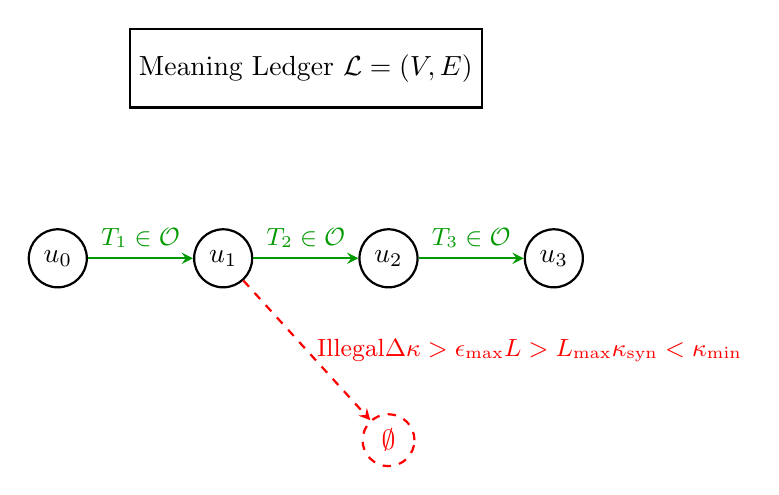
\begin{tikzpicture}[node distance=2.6cm, auto, >=stealth, scale=1.05]

    % LEGEND NODES
    \node[rectangle, draw, thick, minimum width=3.8cm, minimum height=1.0cm]
        (legend) at (0,2.8)
        {Meaning Ledger $\mathcal{L} = (V,E)$};

    % SEMANTIC NODES
    \node[circle, draw, thick] (u0) at (-3,0.5) {$u_0$};
    \node[circle, draw, thick] (u1) at (-1,0.5) {$u_1$};
    \node[circle, draw, thick] (u2) at (1,0.5) {$u_2$};
    \node[circle, draw, thick] (u3) at (3,0.5) {$u_3$};

    % ILLEGAL FAILURE NODE
    \node[circle, draw, red, thick, dashed] (fail) at (1,-1.7) {$\emptyset$};

    % LAWFUL EDGES (LEDGER PATH)
    \draw[->, thick, green!60!black]
        (u0) -- node[above, font=\small]
        {$T_1 \in \mathcal{O}$}
        (u1);

    \draw[->, thick, green!60!black]
        (u1) -- node[above, font=\small]
        {$T_2 \in \mathcal{O}$}
        (u2);

    \draw[->, thick, green!60!black]
        (u2) -- node[above, font=\small]
        {$T_3 \in \mathcal{O}$}
        (u3);

    % ILLEGAL EDGE (REJECTED)
    \draw[->, thick, red, dashed]
        (u1) -- node[right, font=\small]
        {Illegal \\
         $\Delta\kappa > \epsilon_{\max}$ \\
         $L > L_{\max}$ \\
         $\kappa_{\mathrm{syn}} < \kappa_{\min}$}
        (fail);

\end{tikzpicture}

\medskip

\noindent
This diagram encodes the v0.6 ledger geometry:

\begin{itemize}
    \item \textbf{Ledger Graph $\mathcal{L} = (V,E)$}  
    Nodes $u_i$ are semantic states; edges are justified transitions (F.1).

    \item \textbf{Lawful Operators $T_k \in \mathcal{O}$}  
    Each edge corresponds to a contraction-governed operator (IRT, IPU, GBS,
    LRP, EXT) that preserves all invariants (F.2, F.8).

    \item \textbf{Ledger-Closed Path $u_0 \rightarrow u_1 \rightarrow u_2 \rightarrow u_3$}  
    A reasoning chain where every step is ledger-legal (F.4).

    \item \textbf{Illegal Edge to $\emptyset$}  
    Represents a transition with collapse, capture, overload, or drift
    signatures; rejected by the ledger (F.6).

    \item \textbf{Acyclicity}  
    No collapse-inducing or self-referential edges are permitted (F.1).
\end{itemize}

\medskip

\noindent
\textit{This completes G.7 Ledger Geometry.}


% ============================================================
% G.8 PUBLIC-SAFE TRAVERSAL GEOMETRY
% ============================================================

\subsection*{G.8 Public-Safe Traversal Geometry (Safe Corridor Visualization)}

\noindent This diagram visualizes the v0.6 Public‑Safe Traversal Corridor
$\mathcal{C}_{\mathrm{public}}$, the region of the meaning manifold
$\mathcal{M}$ where all public interaction is guaranteed to remain lawful,
curvature‑preserving, identity‑stable, containment‑bounded, and free from
collapse or synthetic capture. The corridor is defined in A.9 and enforced by
runtime legality masks (A.6–A.8) and the Meaning Ledger (Appendix F). All
public‑facing cognitive motion must remain inside this corridor.

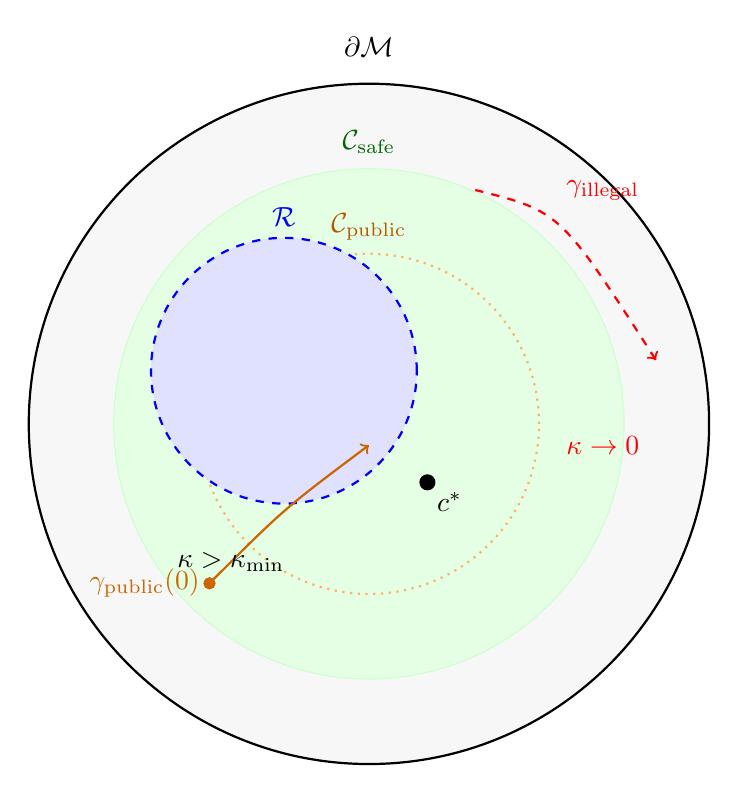
\begin{tikzpicture}[scale=1.35]

    % ============================================================
    % GLOBAL MEANING MANIFOLD
    % ============================================================
    \draw[thick, fill=gray!6] (0,0) circle (3.2cm);
    \node at (0,3.55) {$\partial\mathcal{M}$};

    % ============================================================
    % SAFE REGION
    % ============================================================
    \draw[green!20, fill=green!10] (0,0) circle (2.4cm);
    \node[green!40!black] at (0,2.65)
        {$\mathcal{C}_{\mathrm{safe}}$};

    % ============================================================
    % PUBLIC-SAFE TRAVERSAL CORRIDOR
    % ============================================================
    \draw[orange!60, thick, dotted] (0,0) circle (1.6cm);
    \node[orange!70!black] at (0,1.85)
        {$\mathcal{C}_{\mathrm{public}}$};

    % ============================================================
    % IDENTITY REGION
    % ============================================================
    \draw[blue, thick, dashed, fill=blue!12] (-0.8,0.5) circle (1.25cm);
    \node[blue] at (-0.8,1.95) {$\mathcal{R}$};

    % ============================================================
    % CONTEXT ANCHOR
    % ============================================================
    \filldraw[black] (0.55,-0.55) circle (2pt)
        node[below right] {$c^*$};

    % ============================================================
    % LAWFUL PUBLIC TRAJECTORY
    % ============================================================
    \draw[orange!80!black, thick, ->]
        (-1.5,-1.5) .. controls (-0.8,-0.8) .. (0.0,-0.2);
    \filldraw[orange!80!black] (-1.5,-1.5) circle (1.5pt)
        node[left] {$\gamma_{\mathrm{public}}(0)$};

    % ============================================================
    % ILLEGAL TRAJECTORY (REJECTED)
    % ============================================================
    \draw[red, thick, dashed, ->]
        (1.0,2.2) .. controls (1.8,2.0) .. (2.7,0.6);
    \node[red] at (2.2,2.2)
        {$\gamma_{\mathrm{illegal}}$};

    % ============================================================
    % CURVATURE MARKERS
    % ============================================================
    \node at (-1.3,-1.3) {$\kappa > \kappa_{\min}$};
    \node[red] at (2.2,-0.2) {$\kappa \to 0$};

\end{tikzpicture}

\medskip

\noindent
This diagram encodes the v0.6 public‑safe traversal geometry:

\begin{itemize}
    \item \textbf{Public‑Safe Corridor $\mathcal{C}_{\mathrm{public}}$}  
    Region where all public interaction is guaranteed lawful (A.9).

    \item \textbf{Safe Region $\mathcal{C}_{\mathrm{safe}}$}  
    Runtime curvature‑admissible region (A.6).

    \item \textbf{Identity Region $\mathcal{R}$}  
    Identity‑preserving submanifold (C.2).

    \item \textbf{Context Anchor $c^*$}  
    Anchor for contraction‑governed operator legality (B.1–B.4).

    \item \textbf{Lawful Public Trajectory $\gamma_{\mathrm{public}}$}  
    Motion that remains inside $\mathcal{C}_{\mathrm{public}}$ and preserves:
    

\[
    \text{meaning, identity, geometry, load, curvature, CTL coordinates.}
    \]



    \item \textbf{Illegal Trajectory $\gamma_{\mathrm{illegal}}$}  
    Motion that exits the corridor and approaches collapse or capture geometry;
    rejected by the ledger (F.6).

    \item \textbf{Curvature Markers}  
    Indicators of curvature stability vs. collapse.
\end{itemize}

\medskip

\noindent
\textit{This completes G.8 Public-Safe Traversal Geometry.}


\medskip
\noindent\textit{This outline defines the full v0.6 diagram layer.}
